\section{Introduction}

\begin{figure}
    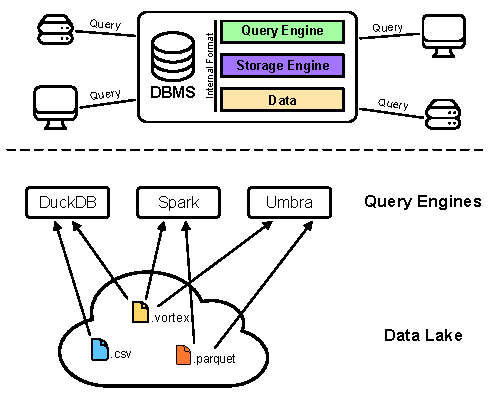
\includegraphics[width=\columnwidth]{figures/evolution_nxm_figure.pdf}

    \Description{Top: A monolithic DBMS with an internal query engine, storage engine, and data layer. Bottom: Multiple query engines (DuckDB, Spark, Umbra) accessing a shared data lake containing files in various formats (Parquet, CSV, Vortex).}

    \caption{(Top) A monolithic DBMS controls its query engine, storage engine, and internal format; clients interact only through queries. (Bottom) In a data lake, multiple query engines access a shared pool of open file formats. Since each must implement a decoder for each format, $N$ engines and $M$ formats require $N \times M$ independent implementations.}

    \label{fig:nxm-problem}
\end{figure}

For decades, database systems functioned as tightly coupled units, with a single system controlling storage format, processing logic, and data access. External systems submitted queries and received results; internal operations remained hidden. With complete control over the physical layout, systems can optimize data storage and processing within their own boundaries. This model was sufficient as long as data did not cross system boundaries~\cite{silberschatzDatabaseSystemConcepts2020}.

However, the volume and variety of collected data have grown drastically. Data now arrives continuously from a growing number of sources, in formats suited to their respective domains rather than to any particular database system. As a result, the database landscape has shifted from a single system controlling all aspects of data management to a heterogeneous, modular ecosystem of specialized systems, each handling a distinct part of the data pipeline using a shared storage layer. Open file formats such as Apache Parquet\footnote{Apache Parquet, \url{https://parquet.apache.org} (accessed: May 22, 2026)} and Apache ORC\footnote{Apache ORC, \url{https://orc.apache.org} (accessed: May 22, 2026)}, stored in data lakes~\cite{armbrustLakehouseNewGeneration2021}, are widely adopted in this context. Beyond these, data scientists increasingly analyze data using domain-specific encodings from fields such as high-energy physics and bioinformatics~\cite{gienieczkoAnyBloxFrameworkSelfDecoding2025}.

Independently, research in data compression and encoding continues to produce formats that surpass established standards for storage efficiency and query throughput. Yet, these advances rarely appear in production systems, because each system must independently implement support for every new format it wants to read~\cite{gienieczkoAnyBloxFrameworkSelfDecoding2025}.

Both trends lead to the same structural problem. Codd's principle of physical data independence~\cite{coddRelationalModelData1970} assumes a system controls its storage format and shields applications from physical details. In a shared storage layer, this does not apply. The data producer determines the format, so any system that reads a format must implement its own decoder. With $N$ systems and $M$ formats, there are $N \times M$ independent implementations to develop and maintain.

This results in higher implementation costs, greater maintenance effort, and increased security risks, as each implementation may contain bugs. For example, a high-severity vulnerability in PostgreSQL's\footnote {PostgreSQL, \url{https://www.postgresql.org} (accessed: May 22, 2026)} JSON support went undetected for over five years~\cite{NVDCVE201715098}. This initial hurdle discourages systems from supporting new formats altogether.

The consequence is a self-sustaining cycle: systems do not adopt a new file format because its user base is too small, and the user base remains small because the format lacks support. Gienieczko et al.\ (2025) identify this as a core structural problem because an encoding must be popular enough to justify support, but cannot gain popularity without broad support.

This dynamic leads to format ossification, in which datasets use outdated formats simply to remain compatible, even when better encodings exist~\cite{kuiperQueryEnginesGatekeepers2025}. Changing formats is difficult because it risks breaking compatibility with many systems that use older specifications.

But what could solve this combinatorial integration burden? An abstraction layer between storage formats and processing systems reduces the $N \times M$ problem to $N + M$. Each system implements the interface once, and each format provides a single implementation against it. Gienieczko et al.\ (2025) propose exactly this and present AnyBlox as their realization.